%!TEX root = ../../thesis.tex

\section{A minimalist proof}
\label{chapter:limitations:proof}

It is of paramount importance to understand the properties of our algorithm, and to be able to have some certitude about its convergence and accuracy properties. The work presented in this thesis neglected this aspect and relied only on empirical evaluation. The next step for a motivated person it to work on a formalism of our problem and to derive some useful proof about some properties of the algorithm. In the following of this section we present a minimalist proof of the principle of our algorithm under extremely narrow condition.

\subsection{Problem and assumptions}

We consider a robot in a discrete state and action world. A teacher is providing feedback instruction to the robot through the use a simple interface with two buttons, one button for ``correct'' and one button for ``incorrect''. But the mapping between the buttons and the meanings is unknown to the robot at start.

This simplified setting, where the signals provided by the user, is certainly the first scenario that should have been considered in this work. Indeed it allows to study specific details of the algorithm in more details, without the influence of the classifier properties and  assumptions.

As for all our scenario, we assume that the user is coherent and uses one button for one meaning, and always the same button for the same meaning. Therefore, as exemplified in Figure~\ref{fig:proofmapping} the mapping between symbolic signals and their meaning can only be of two forms. 

\begin{figure}[!htbp]
\centering
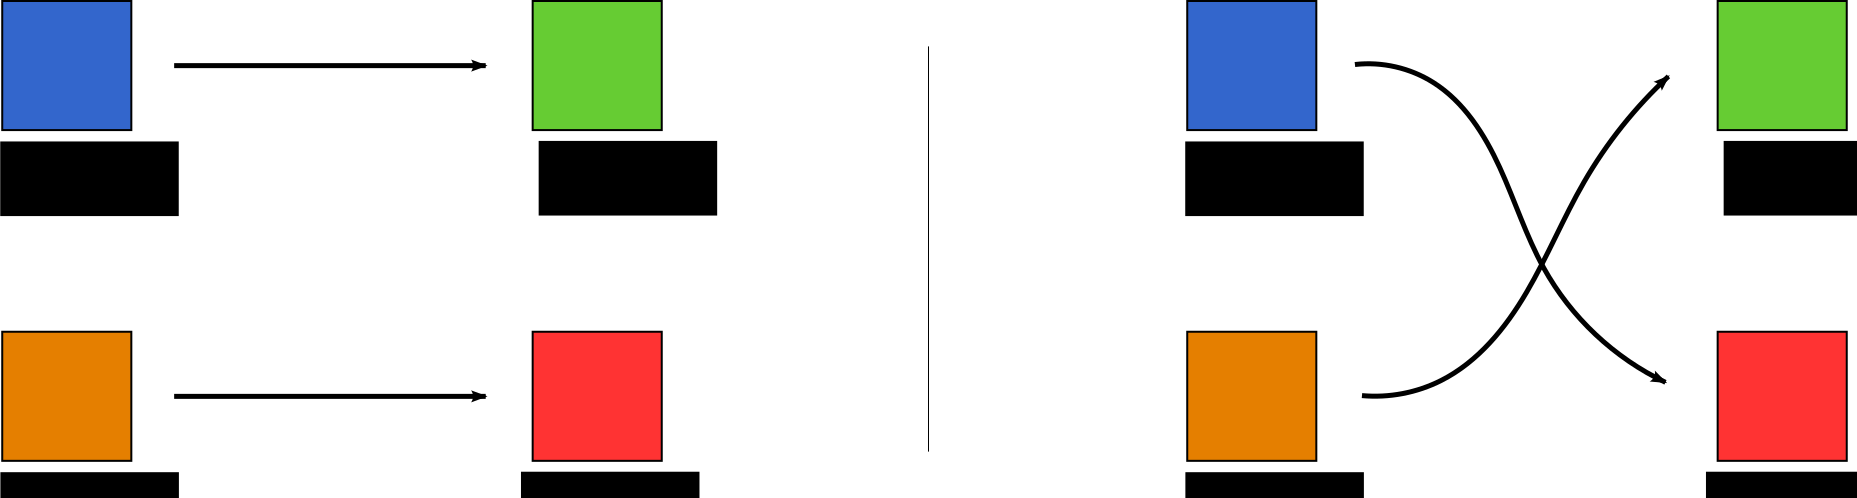
\includegraphics[width=\columnwidth]{\visualspdf/proof/mappings.pdf}
\caption{The two possibles button to meaning mapping.}
\label{fig:proofmapping}
\end{figure} 

We further assume the robot is provided with a set of task hypothesis ($\xi_1,\ldots,\xi_T$), represented by their associated policies ($\pi_1, \ldots, \pi_T$). This set includes the task $\hat{\xi}$, the teacher as in mind, and when the robot performs a non-optimal action according to the optimal policy $\hat{\pi}$ associated to this task, the teacher presses the button associated to the ``incorrect'' meaning. Respectively pressing the  the button associated to the ``correct'' meaning for an optimal action. Finally we assumed that the teacher never makes teaching mistakes.

We define a number of terms that will simplify the notation in further subsections. $nS$ is the number of states in the environment, $nA$ is the number of actions available to the robot, and $nSA$ is the number of state-action pairs an agent can visit, which is simply $nS * nA$. We note as $diff(\pi_t, \pi_u)$ the number of optimal state-action pairs that differs between the optimal policies $\pi_t$ and $\pi_u$ respectively associated to the task $\xi_t$ and $\xi_u$. Therefore the ratio of optimal state-action pairs that differs between two task hypothesis is denoted as $\frac{diff(\pi_t, \pi_u)}{nSA}$. 

The $diff()$ function logically outputs $0$ when comparing one task to itself, i.e. $diff(\pi_t, \pi_t) = 0$. A ratio of 0 between two tasks means they are the same. And, as discussed in chapter~\ref{chapter:lfui:symmetries}, a ratio of 1 means the two tasks are symmetric which means whatever the action the robot will choose, the meaning inferred according to the first task will be the opposite of the meaning inferred according to the second task. This property, as will be seen in our minimalist proof, do not allow to differentiate between two symmetric task.


\subsection{Illustration}

Before describing our simple proof, it is important to have an intuition on the relation between the buttons and the meanings in different condition. We will consider again our T world scenario as an illustration (see chapter~\ref{chapter:lfui:example}).


Figure~\ref{fig:proofsymbolic} shows all possible button presses sequence expected from the teacher in different condition. On top are the state-action pair considered (a). (b) and (c) lines represent the expected meanings for each of the state-action pairs and according to the hypothesis G1 (b) or G2 (c). (d) and (e) lines represent the possible button presses sequence of the teacher when teaching hypothesis G1 and considering the two possible mappings. Respectively (f) and (g) for hypothesis G2.

\begin{figure}[!htbp]
\centering
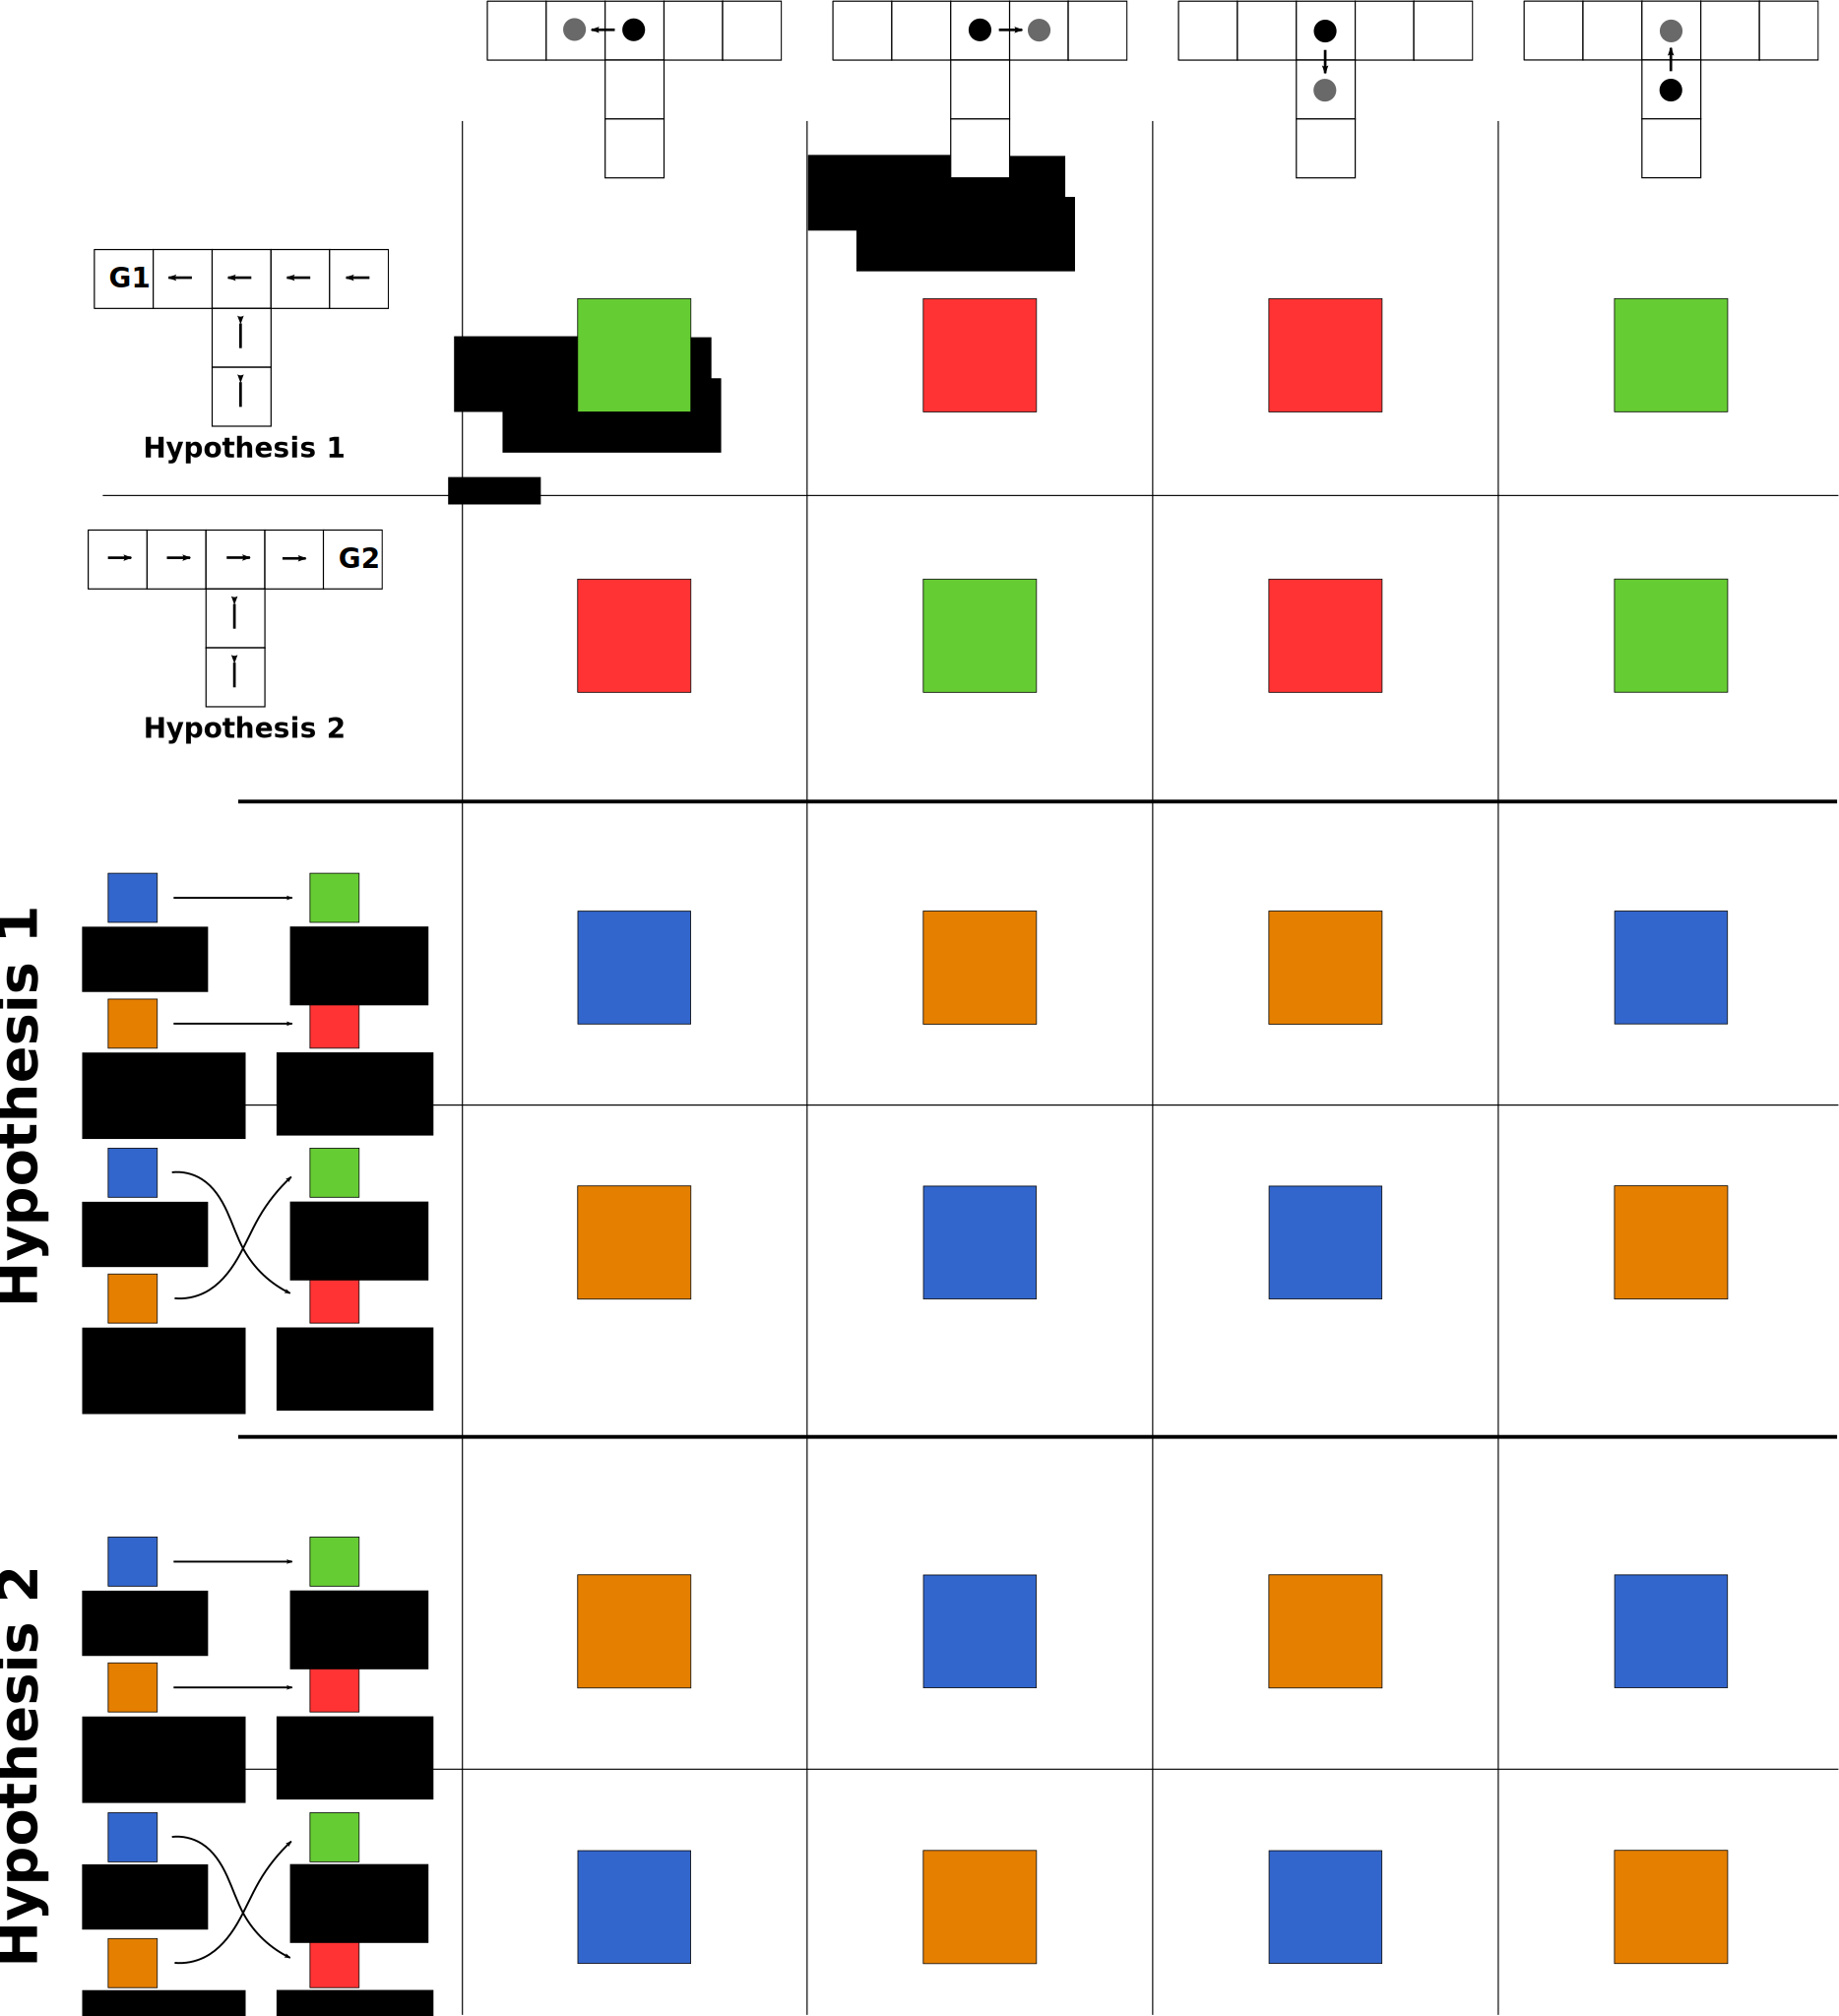
\includegraphics[width=\columnwidth]{\visualspdf/proof/symbolic_feedback.pdf}
\caption{Illustration of the teacher's button presses for several state-action pairs. On top are the state-action pair considered (a). (b) and (c) lines represent the expected meanings for each of the state-action pairs and according to the hypothesis G1 (b) or G2 (c). (d) and (e) lines represent the possible button presses sequence of the teacher when teaching hypothesis G1 and considering the two possible mappings. Respectively (f) and (g) for hypothesis G2.}
\label{fig:proofsymbolic}
\end{figure} 

First, before entering into more details, given the extensive number of assumptions defined, for the simple example of Figure~\ref{fig:proofsymbolic} it would be easy to find the correct hypothesis by visiting only two state-action pairs. Indeed as taking an action in the trunk of the T will produce similar responses from the teacher for all hypothesis, and that the user if not making teaching mistakes and is coherent in its use of the buttons, we would instantaneously know the meaning of the button pressed and therefore the meaning of the other button. Then taking an action in the top bar of the T would allow us to differentiate between G1 and G2. However we will not exploit this type of properties for our proof and we remind that in all the experimental scenarios presented in this thesis, there were no state-action pairs that allowed for an unequivocal interpretation of a signal.

Now, for the purpose of our demonstration, we should read this figure by comparing lines (d), (e), (f), and (g) with the expectation from lines (b) and (c). We will denote $B$ the blue button, O the orange button, $C$ the ``correct'' meaning (the green patch), and $W$ the ``incorrect'' meaning (the red patch, $W$ for wrong). For example, let's imagine we receive the sequence of presses of line (d) which we note $[B,O,O,B]$. For hypothesis 1 (G1) we expected $[C,W,W,C]$, and for hypothesis 2 (G2) we expected $[W,C,W,C]$. 

Given this two possible interpretation we can build a statistical model for the signal to meaning mapping. For G1, we obtain the following model $p(C|B, G1) = \frac{2}{2} = 1$, $p(C|O, G1) = \frac{0}{2} = 0$, and $p(W|B, G1) = \frac{0}{2} = 0$, $p(W|O, G1) = \frac{2}{2} = 1$. To simplify notation we note $[1,0]_{B,G1}$ and $[1,0]_{O,G1}$ the model for each button where the first element of the vector is the probability associated to the ``correct'' meaning and the second is the one associated to the ``incorrect'' meaning. And the underscript details the button and the task considered. Using the same reasoning, again for line (d) but for hypothesis G2, the classifier is: $[0.5,0.5]_{B,G2}$ and $[0.5,0.5]_{O,G2}$.

In this thesis, as we were not considering symbolic signals, we used a metric that compares the expectation from the frame (i.e. lines (b) and (c)) with a classifier associated to each task. Let's use Equation~\ref{eq:matchingoverfitting} to compute the likelihood for each task. For G1 we obtain:
%
\begin{eqnarray}
\L(G1) &=& \left((1\times1)+(0\times0)\right)\left((0\times0)+(1\times1)\right)\left((0\times0)+(1\times1)\right)~\ldots  \nonumber \\
&& \ldots~\left((1\times1)+(0\times0)\right)  \nonumber \\
&=& 1 \nonumber
\end{eqnarray}

And for G2 we obtain:
%
\begin{eqnarray}
\L(G2) &=& \left((0.5\times0)+(0.5\times1)\right)\left((0.5\times1)+(0.5\times0)\right)~\ldots  \nonumber \\
&& \ldots~\left((0.5\times0)+(0.5\times1)\right)\left((0.5\times1)+(0.5\times0)\right) \nonumber \\
&=& 0.0625 \nonumber
\end{eqnarray}

By normalizing the likelihoods, we obtain the probability of each task: $p(G1) \approx 0.94$ and $p(G2) \approx 0.06$. We see that our measure of likelihood is able to identify the correct task. The same process can be repeated for each cases (i.e. (e), (f), and (g)) and will always identify the correct hypothesis. 

Given this explanation, we are ready to move on for the actual proof, in which to simplify the proof, we will add an additional assumption.

\subsection{The proof}

In order to make the proof simple, we assume each hypothetic policy has an equal number of optimal state-action pairs than of non-optimal state-action pairs. Therefore when the agent has visited once all the state-action pairs, it has collected, for each hypothesis, the same amount of signals with label ``correct'' than with label ``incorrect''. As a consequence, this properties ensures that the signal to meaning model for each class (i.e. for $C$ and $W$) are symmetric. 

We can explain this effect as follows. First, for all hypothesis this assumption ensure that, when the agent has visited once all the state-action pairs, the user will have pressed as many time the blue button than the orange button, exactly $\frac{nSA}{2}$ times. And the same assumption ensures that whatever the task considered the number of ``correct'' and ``incorrect'' labels will be the same. However the number of blue button presses associated to ``correct'' or ``incorrect'' labels remains undefined and depends on the overlap between the true unknown policy taught by the teacher and the one considered by the agent in the labeling process. 

Therefore, we can evaluate the possible mapping models based on the difference in policies between the optimal task and any hypothetic task using our $diff()$ function defined earlier. For a given task $\xi_t$ we can compute the ratio of optimal state-action pairs that are the same as for the true task $\hat{\xi}$, which we denote $\Upsilon_{\xi_t} = \frac{nSA - diff(\pi_t, \hat{\pi})}{nSA}$. Obviously the agent will never have access to this information and we only use this measure for our proof.

Given our previously defined assumption, and assuming the agent visited all state-action pairs once, if the user uses the blue button to mean ``correct'', then the blue signal model will be $[\Upsilon_{\xi_t},1-\Upsilon_{\xi_t}]_{B,\xi_t}$. Which implies the orange button mapping is $[1-\Upsilon_{\xi_t},\Upsilon_{\xi_t}]_{O,\xi_t}$. Respectively, if the user uses the blue button to mean ``incorrect'', then the blue signal model will be $[1-\Upsilon_{\xi_t},\Upsilon_{\xi_t}]_{B,\xi_t}$. Which implies the orange button mapping is $[\Upsilon_{\xi_t},1-\Upsilon_{\xi_t}]_{O,\xi_t}$. 

As there is the same number of ``correct'' and ``incorrect'' expected labels, we can factorize the likelihood equation as follows (see appendix~\ref{appendix:proof}):
%
\begin{eqnarray}
\L(\xi_t) &=& \Upsilon_{\xi_t}^{nSA.\Upsilon_{\xi_t}} \times (1-\Upsilon_{\xi_t})^{nSA.(1-\Upsilon_{\xi_t})}
\label{eq:likelihoodproof}
\end{eqnarray}

Note that this equation is the same whatever the button chosen by the user to mean ``correct''. We can check our previous likelihood estimate in our simple example of Figure~\ref{fig:proofsymbolic} considering the 4 state-action space visited are the only one available in the world, and considering we receive button presses as in line (d). We obtain the same likelihoods as the one derived in the first subsection, i.e. $\L(G1) = 1^{1\times4} \times 0^{0\times4} = 1$ and $\L(G1) = 0.5^{0.5\times4} \times 0.5^{0.5\times4} = 0.5^4 = 0.0625$.

Let's plot the likelihood function with respect to the full range of value that $\Upsilon_{\xi_t}$ can take, i.e. between 0 and 1. We consider that $nSA = 1$ for now. Obviously such a value of $nSA$ is impossible in practice given our assumptions, we need as many optimal and non-optimal state-action pair, which means that $nSA$ must be an even number. However, now that we have our theoretical estimate of the likelihood function we shall study its properties in a theoretical way. Additionally, our equation is only valid if the agent visited all state-action pair but for the sake of our analysis, we consider that the value of $nSA$ represents the number of state-action pair visited by the agent. Moreover, there exist a relation between the number of state-action pair and the discrete set of value that $\Upsilon_{\xi_t}$ can take given our assumptions, but for the sake of the analysis we consider the full range of value between 0 and 1.

Figure~\ref{fig:prooflikelihoodone} shows the likelihood function for $nSA = 1$. As expected the likelihood value is higher for the correct task, i.e. when $\Upsilon_{\xi_t} = 1$, and decrease as the number of state-action pairs that differ increase, i.e. when $\Upsilon_{\xi_t}$ decrease. However this function holds an interesting property, which is that once more than half of the optimal state-action pair differs with the true task, the function increases again. Until is reaches a point where none of the optimal state-action pair of the task are the same as for the true task. This specific case is what we called symmetric task hypothesis, where the symmetric interpretation of the feedback signals is as likely as  the correct interpretation of the signals. Indeed none of the state-action pairs allow to break this symmetry for the feedback frame. 

Therefore, given all the assumptions considered, if the agent is provided with a set of task hypothesis, that included the correct task $\hat{\xi}$ but does not include any symmetric hypothesis --- which means all tasks hold the following property $\Upsilon_{\xi_t} > 0$ ---, we can guarantee that if the teacher visits all state-action pairs once, the user intended task $\hat{\xi}$ --- which hold the property $\Upsilon_{\xi_t} = 1$ --- will have the greater likelihood. In other words: $\L(\hat{\xi}) > \L(\xi_t)$ if $\Upsilon_{\xi_t} \in~]0,1[$.

\begin{figure}[!htbp]
\centering
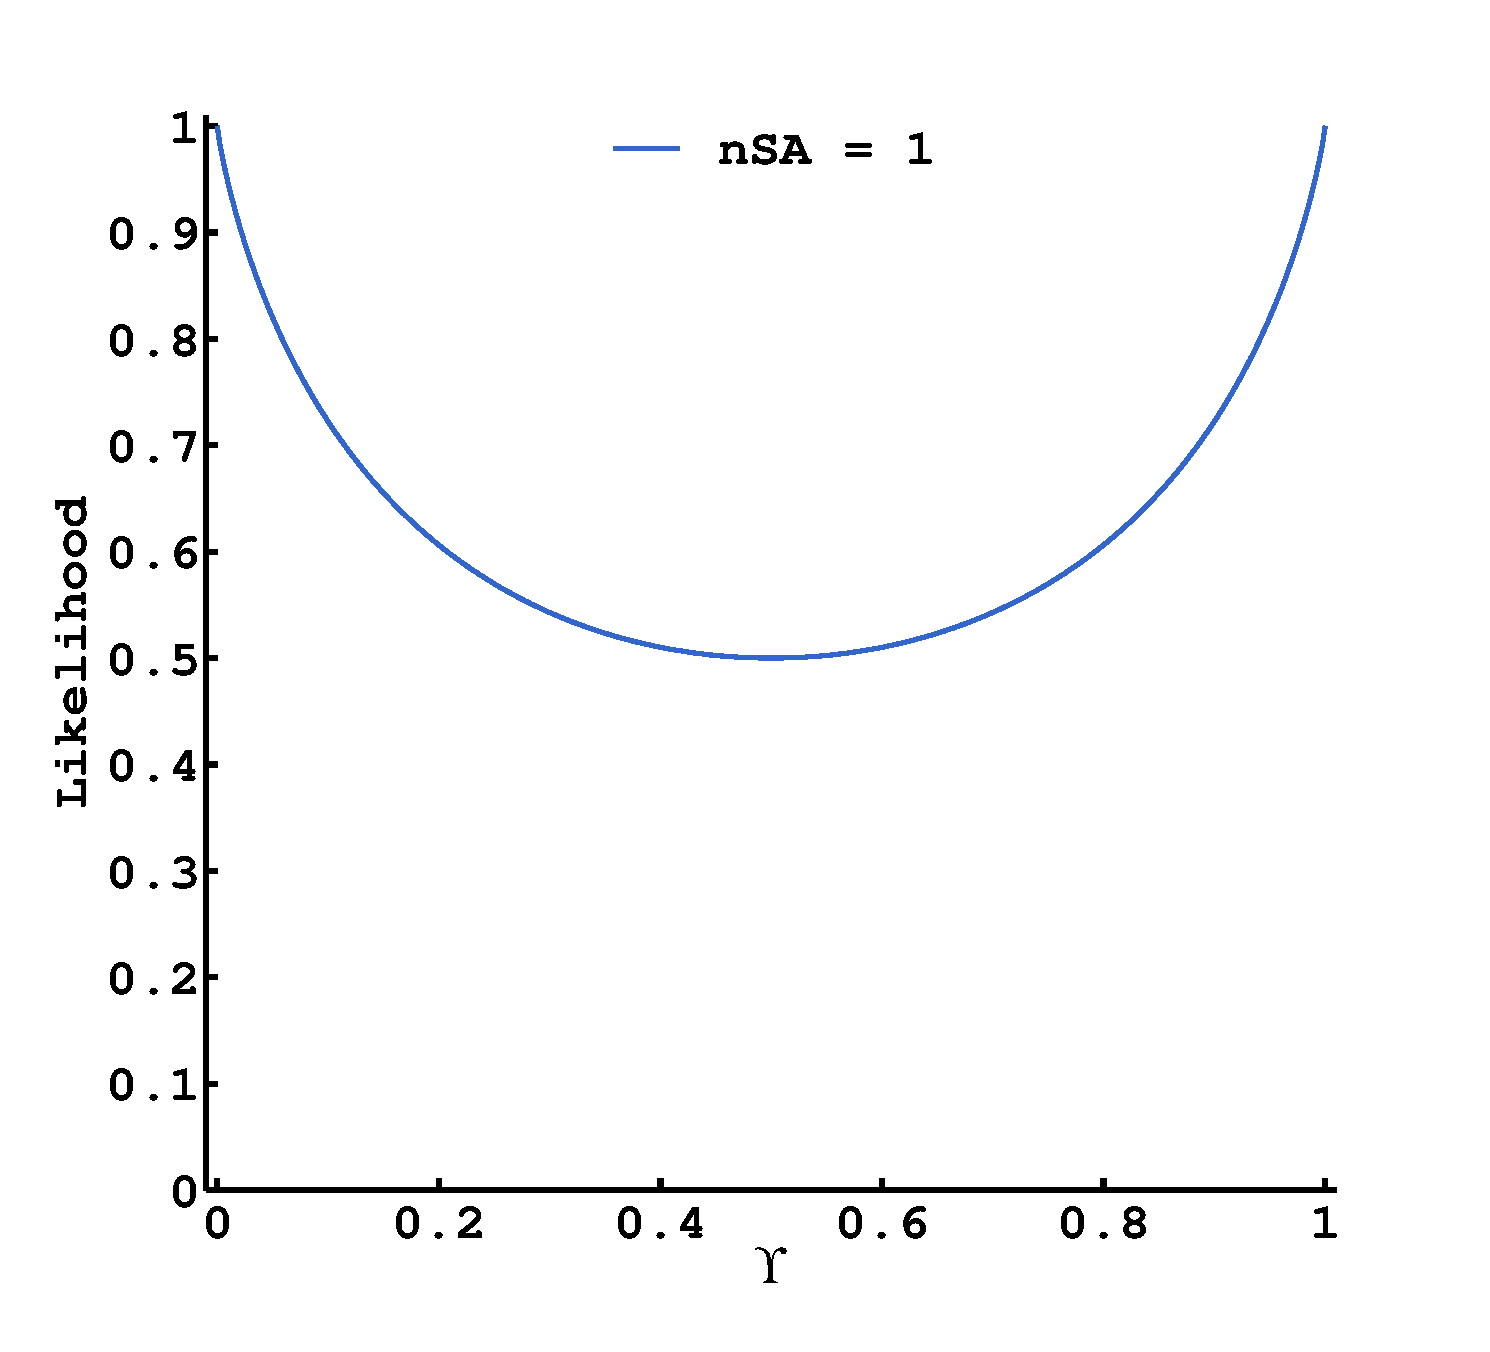
\includegraphics[width=\plotsize\columnwidth]{\imgpath/proof/likelihoodOne}
\caption{The likelihood function of Equation~\ref{eq:likelihoodproof} for $nSA =1$.}
\label{fig:prooflikelihoodone}
\end{figure}

We now discuss the problem of estimating our confidence that one task is a better candidate than an other one. Of course, in this setting, given the strong assumption that the user is never making mistakes, such confidence mechanism is not needed. However, we have seen in previous chapter that deciding when to stop is a critical part of the algorithm. The simplest method consist of normalizing the likelihood for each task defining a probability threshold above which a task is considered as the correct one. If we consider for example 10 task hypothesis with different values of $\Upsilon$, normalizing the likelihood when $nSA = 1$ won't produce a very sharp probability distribution on task. All task will roughly share the same probability. However, when visiting more and more states, the likelihood function becomes more and more sharp and only normalizing likelihoods will split the hypothesis apart. In the limit, when $nSA \rightarrow +Inf$, only the hypothesis with a better value of $\Upsilon$ (i.e. closer to 0 or 1) will reach a probability of 1.

\begin{figure}[!htbp]
\centering
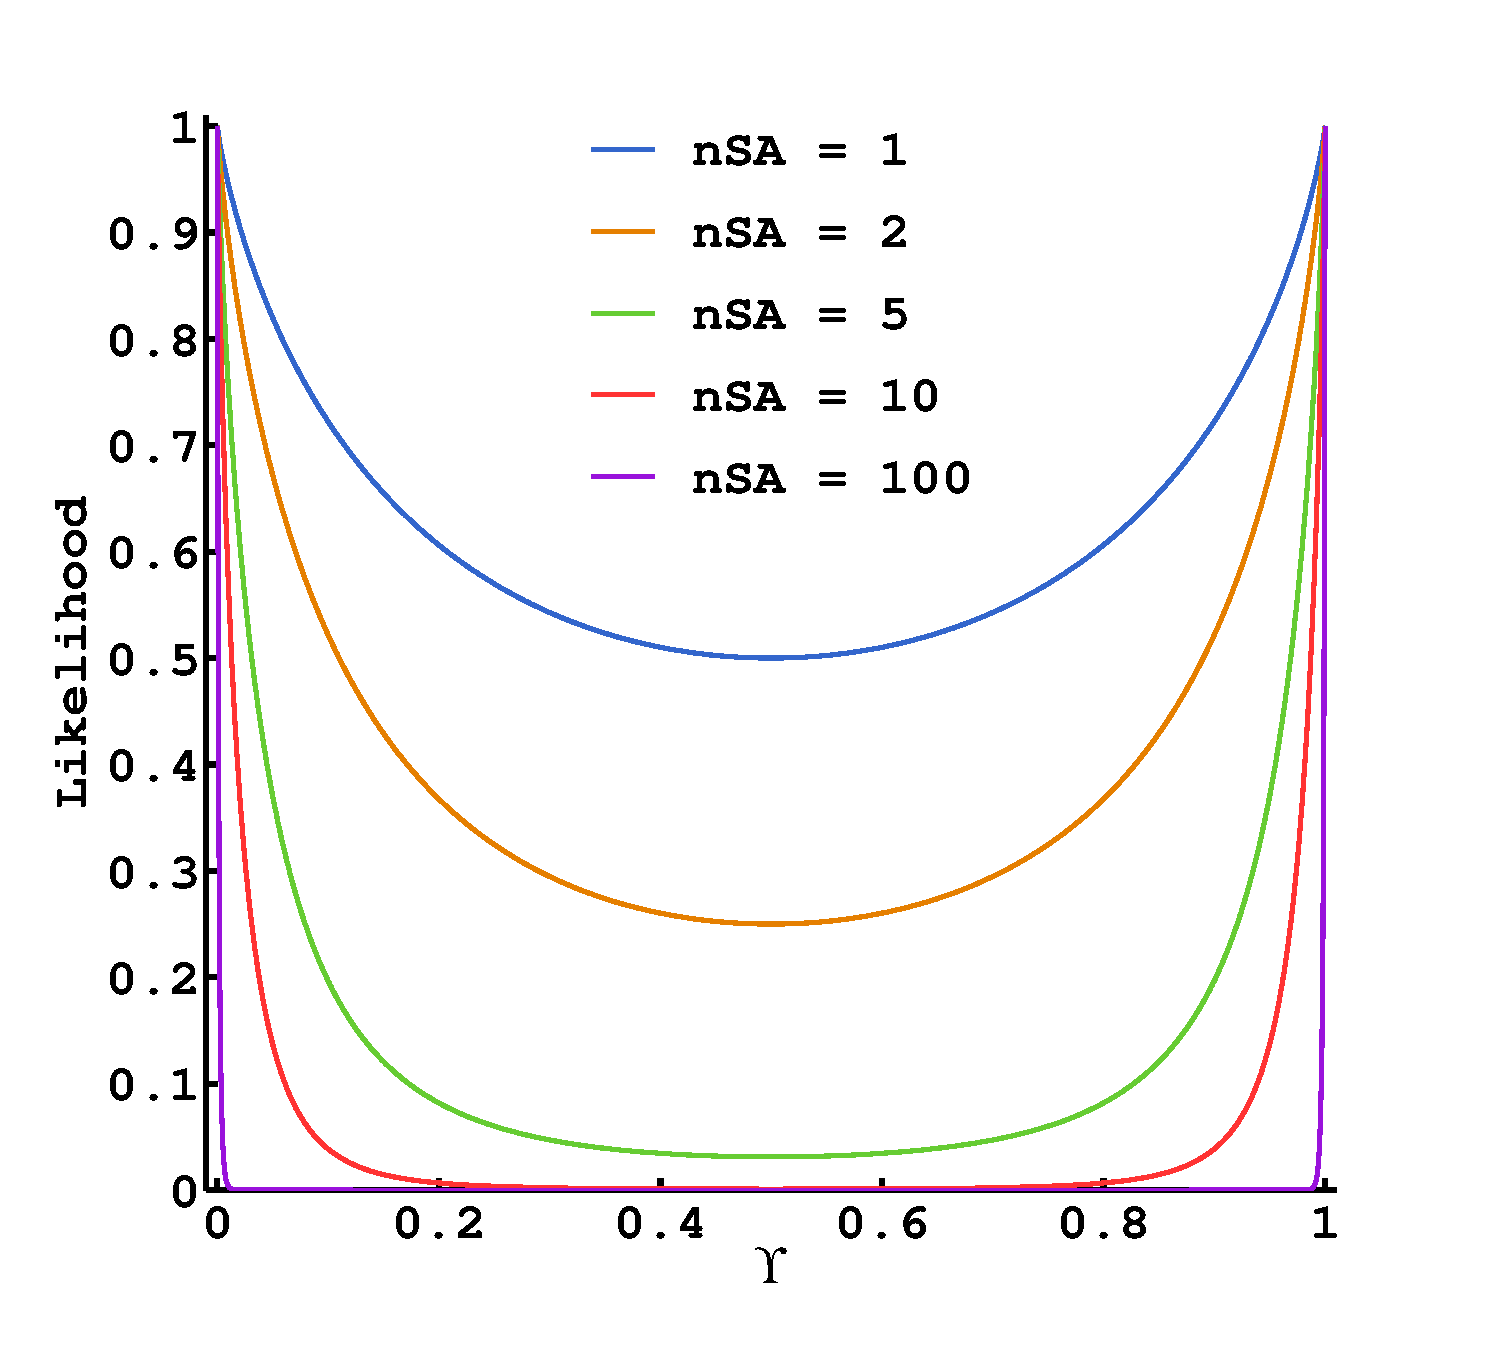
\includegraphics[width=\plotsize\columnwidth]{\imgpath/proof/likelihoodMany}
\caption{The likelihood function of Equation~\ref{eq:likelihoodproof} for $nSA =1,2,5,10,100$. The more we have collected evidence, the more the difference is sharp between task hypothesis.}
\label{fig:prooflikelihoodmany}
\end{figure}

This model allows to understand in more conceptual terms some properties of our algorithm. And in practice very few of the assumption considered are applicable in our experimental setups.

Finally, for illustration purpose, we present a world holding all our assumption properties, we named it the clock world (see Figure~\ref{fig:clockworld}). This world has 12 states, which we represent as the hours on a clock. The agent has two actions available: turning clockwise or counter-clockwise. The user wants the agent to reach one of 12 states. This world is the extension of the line word but where the line loops on itself.

\begin{figure}[!htbp]
\centering
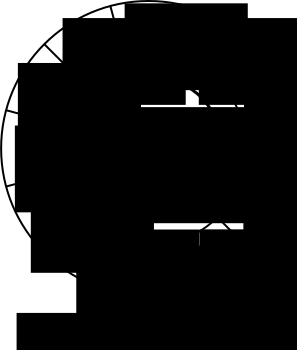
\includegraphics[width=0.3\columnwidth]{\visualspdf/proof/clockworld.pdf}
\caption{Illustration of the clock world. The agent has two actions available: turning clockwise or counter-clockwise. The user wants the agent to reach one of 12 states.}
\label{fig:clockworld}
\end{figure} 

\subsection{Why not using the entropy of the meaning models?}

We continue here the discussion about the difference between the method detailed in this thesis work and the method presented in section~\ref{chapter:limitations:overlap}. In section~\ref{chapter:limitations:overlap}, we tried to differentiate the task by looking at the overlap of the model for each class. In other words, we tried to evaluate the uncertainty of the signal model fitted for each task, and we selects the one that as lower uncertainty.

We can do the same in our simple example, indeed, as we assumed that the user is coherent in his button presses, the task whose associate button presses model is the less uncertain is the more likely to be the correct one. Given the history of interaction, we can model the button presses of the user as Bernoulli variables, which can take only two values ``correct'' or ``incorrect'', such as a coin flipping problem. Following the previous development, we can compute the probability that the user will press the blue button to mean ``correct'', which is $\Upsilon_{\xi_t}$ (or $1-\Upsilon_{\xi_t}$ if the orange button is used for ``correct'').

The binary entropy function, denoted $H_{\mathrm b}(p)$, is the entropy of a Bernoulli process with probability of success p, and can be computed as follows:

\begin{eqnarray}
H_{\mathrm b}(p) = -p\log_2(p) - (1-p)\log_2(1-p) 
\label{eq:likelihoodentropy}
\end{eqnarray}

The binary entropy function is shown in Figure~\ref{fig:prooflikelihoodentropy}. As one would expect the shape of the entropy function holds similar properties than our likelihood Equation~\ref{eq:likelihoodproof}.
    
\begin{figure}[!htbp]
\centering
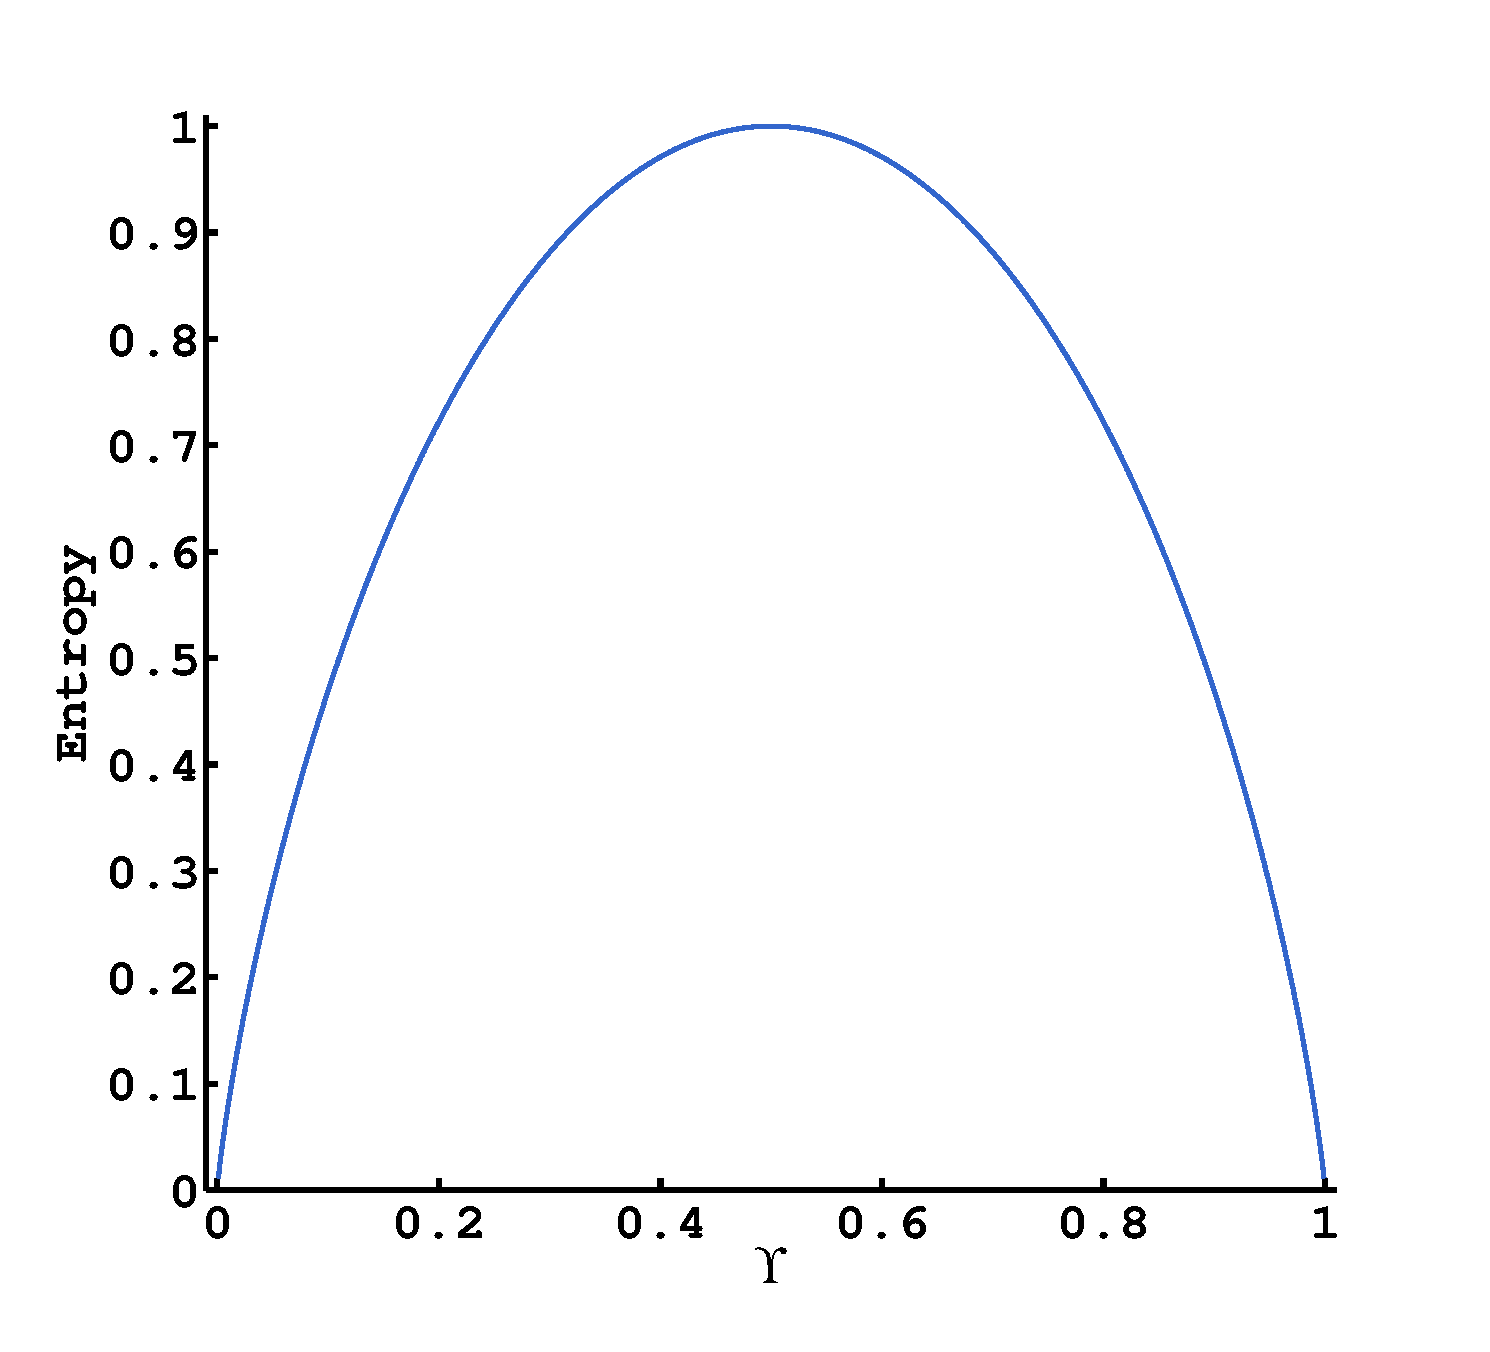
\includegraphics[width=\plotsize\columnwidth]{\imgpath/proof/entropy}
\caption{The binary entropy function.}
\label{fig:prooflikelihoodentropy}
\end{figure}

This method allow us to rank correctly our task hypothesis with respect to the uncertainty of their estimated models. However, this function will not ``sharpen'' as the likelihood Equation~\ref{eq:likelihoodproof} when the agent visit more and more states. The only change will result in a better approximation of the Bernoulli process modeling the button presses.

Therefore, this method alone is not enough to estimate which task is the correct one as one should also measure the uncertainty of the measure of uncertainty. To do so, we propose to use beta distribution, which is the conjugate prior probability distribution for the Bernoulli distributions. A beta distribution would describe the initial knowledge concerning probability of button presses and would be updated as new information comes in. Finally, by comparing between the beta distribution associated to each task, we could expect to find a suitable measure of task confidence. The interested readers may refer to \cite{montesano2012active} for a practical robotic example using this process.

\subsection{Discussion}

While it is always interesting and useful to formulate proof of algorithm, the restricted assumption used in this section makes it impossible to use this results in practical scenario. But we note that our experimental results shows that our algorithm can work with fairly good performance on different scenarios using continuous signals as noisy as EEG signals.

I personally have very few experience in making proof for such kind of problems and it may be useful to pursue in that direction by releasing some of the assumptions steps after steps. Starting with the assumption that all hypothesis have half of their state-action pair optimal and half non-optimal, and progressively accounting for some teaching mistakes. Reaching that level of proof would already offer some guarantees for simple scenarios using discrete state, discrete action, and symbolic signals, but under more realistic teaching conditions.
